% Fixture: two-column-midpage
% Two-column text (multicol) on A4 with full-width elements in the MIDDLE of
% a page: a band of two columns, then a full-width figure, then another band
% of two columns below it. The correct reading order is band 1 left, band 1
% right, the wide figure, band 2 left, band 2 right -- which neither a
% top-to-bottom sort nor a "whole left column first" rule produces.
%
% Column breaks are forced with \columnbreak and every band is its own
% multicols environment, so the column of each paragraph is fixed by this
% source.
\documentclass[10pt]{article}
% Shared settings for every Tourmaline fixture. \input this right after
% \documentclass.
%
% Reproducible output: no creation date, no random trailer id, no pdfTeX
% banner, so rebuilding with the same TeX Live gives byte-identical PDFs.
\pdfinfoomitdate=1
\pdftrailerid{}
\pdfsuppressptexinfo=-1
% Map every glyph (including the fi/fl/ffi ligatures) to Unicode so that
% text extraction does not depend on font-specific guesswork.
\input{glyphtounicode}
\pdfgentounicode=1

\usepackage[a4paper,margin=22mm]{geometry}
\usepackage{multicol}
\usepackage{caption}
\usepackage{tikz}
\setlength{\columnsep}{8mm}

\title{Wide Elements Between Column Bands}
\author{Dana Filler\\ Laboratory of Sample Layouts}
\date{}

\begin{document}
\maketitle

\begin{abstract}
Some journals place wide figures, tables and equations in the middle of a
page, with two columns of text above them and two more below. A reader
finishes both upper columns before looking at the wide element, and only
then continues with the lower columns.
\end{abstract}

% ------------------------------------------------------------ page 1, band 1
\begin{multicols}{2}
\section{Background}

Columns in the upper band are short, because the wide figure that follows
them takes up the middle of the page. The left column of this band ends
with this sentence.

\columnbreak

The right column of the upper band continues the argument. It must be read
after the left column of the same band, but before the caption of the
figure below it.
\end{multicols}

% -------------------------------------------------------- page 1, wide figure
\begin{center}
  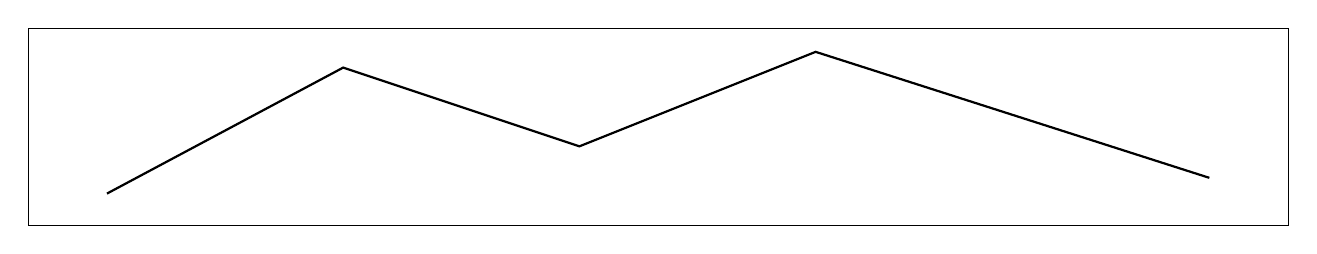
\begin{tikzpicture}[x=10mm,y=10mm]
    \draw (0,0) rectangle (16,2.5);
    \draw[thick] (1,0.4) -- (4,2.0) -- (7,1.0) -- (10,2.2) -- (15,0.6);
  \end{tikzpicture}
  \captionof{figure}{A wide figure placed between two bands of columns.
  Its caption spans the full width of the text block.}
  \label{fig:wide}
\end{center}

% ------------------------------------------------------------ page 1, band 2
\begin{multicols}{2}
\section{Observations}

The lower band starts again in the left column, directly below the wide
figure. A reader who sorted the page by column alone would jump here too
early, straight after the upper left column.

\columnbreak

The right column of the lower band is the last text on the first page.
Anything that follows belongs to the next page of the document.
\end{multicols}

\clearpage

% ------------------------------------------------------------ page 2, band 1
\begin{multicols}{2}
\section{A wide equation}

Displayed material that is too long for one column is often set across the
full width, splitting the columns above and below it in the same way as a
wide figure does.

\columnbreak

The same rule applies: finish both columns above the display, read the
display, then continue in the left column underneath it.
\end{multicols}

\begin{equation}
  \Phi(x) = \sum_{i=1}^{n} \alpha_i \exp\!\left(-\frac{(x-\mu_i)^2}{2\sigma_i^2}\right)
  + \sum_{j=1}^{m} \beta_j \cos(\omega_j x + \varphi_j) + \gamma x^2 + \delta
  \label{eq:wide}
\end{equation}

% ------------------------------------------------------------ page 2, band 2
\begin{multicols}{2}
\section{Closing remarks}

Mid-page wide elements are less common than wide floats at the top of a
page, but they appear in several journal styles.

\columnbreak

A full-width paragraph may also close the page, as the acknowledgement below
does.
\end{multicols}

\noindent\textbf{Acknowledgements.} This full-width paragraph follows both
columns of the lower band and is read last on the page.

\end{document}
